\documentclass[10pt,a4paper]{article}
\usepackage[margin=18mm]{geometry}
\usepackage[T1]{fontenc}
\usepackage{lmodern,graphicx,booktabs,array,amsmath,amssymb,microtype,xcolor,caption,fancyhdr}
\usepackage[hidelinks]{hyperref}
\hypersetup{pdftitle={EyeCode Research Entry Task - Mobile Manipulation},pdfauthor={Bui Hoang Linh}}
\setlength{\parindent}{0pt}
\setlength{\parskip}{4pt}
\renewcommand{\arraystretch}{1.12}
\captionsetup{font=small,skip=4pt}
\pagestyle{fancy}\fancyhf{}\fancyhead[L]{\small EyeCode Research Entry Task}\fancyhead[R]{\small Mobile Manipulation}\fancyfoot[C]{\thepage}
\setlength{\headheight}{14pt}
\newcommand{\artifact}[1]{\texttt{\small #1}}
\begin{document}
\begin{center}
{\LARGE\bfseries Mobile Manipulation: Simulation and Research Reproduction}\\[5pt]
{\large EyeCode Research Entry Task --- Technical Report}\\[4pt]
B\`ui Ho\`ang Linh \quad | \quad October 2026
\end{center}
\textbf{Scope and main findings.} This submission combines ROSOrin Pro mapping/navigation with small-scale studies of HoMMI and MoManipVLA. ROSOrin completed 21 exploration waypoints and saved a map subsequently used by single-goal and multi-point Nav2 actions. A controlled SLAM replay identified a configuration change that reduced mean pose error from 2.07\,m to 0.013\,m. The official HoMMI policy was trained on 30 Laundry demonstrations and evaluated offline. A reduced MoManipVLA planner achieved 32/60 successes; selecting feasible candidates first increased this to 40/60. These research results test individual mechanisms, rather than reproduce the original robot benchmarks.

\section*{1. Part 1: ROSOrin Pro simulation}
\textbf{Environment.} Following Hiwonder's simulation documentation [1], the robot ran in the RoboCup Home world on Ubuntu 22.04.4, ROS 2 Humble, Gazebo Fortress 6.16 and Nav2 1.1.14. The VirtualBox guest had six vCPUs and 6\,GB RAM; the host was an i5-13420H laptop with approximately 14\,GB RAM. Mesa software rendering required a logged-in X display even when the 3D Gazebo client was disabled. No physical robot was used.

\textbf{Pipeline.} Gazebo's MecanumDrive consumes bridged \artifact{/cmd\_vel}. Its OdometryPublisher supplies \artifact{/odom} and \artifact{odom $\rightarrow$ base\_footprint}; the drive's duplicate odometry is isolated on \artifact{/wheel/odom}. The bridge also carries \artifact{/clock} and LiDAR \artifact{/scan}. All nodes use simulation time. SLAM Toolbox owns \artifact{map $\rightarrow$ odom} during mapping; after map saving, AMCL becomes the sole owner. Nav2 uses Navfn and Regulated Pure Pursuit (RPP), with a velocity smoother.

\begin{center}\small
\begin{tabular}{p{.29\linewidth}p{.65\linewidth}}\toprule
Required capability & Measured outcome in the final recorded session\\\midrule
Control and LiDAR & 0.10\,m forward command: 0.1005\,m measured; turn: 0.829\,rad. LiDAR: 270 beams, 10\,Hz, approximately 260 finite returns per scan.\\
SLAM exploration & Four routes, 21/21 waypoints, 52.4\,m travelled; mean/max pose error 0.023/0.058\,m against simulation ground truth.\\
Saved map & 203$\times$162 cells, 0.05\,m/cell; 27,382 free, 1,921 occupied and 3,583 unknown cells.\\
Single goal on saved map & Nav2 status 4; final error 0.103\,m / 0.005\,rad; 39.8\,s including initialization.\\
Four ordered waypoints & Status 4, no missed waypoints; final error 0.141\,m / 0.039\,rad; 123\,s.\\\bottomrule
\end{tabular}\end{center}

\begin{center}
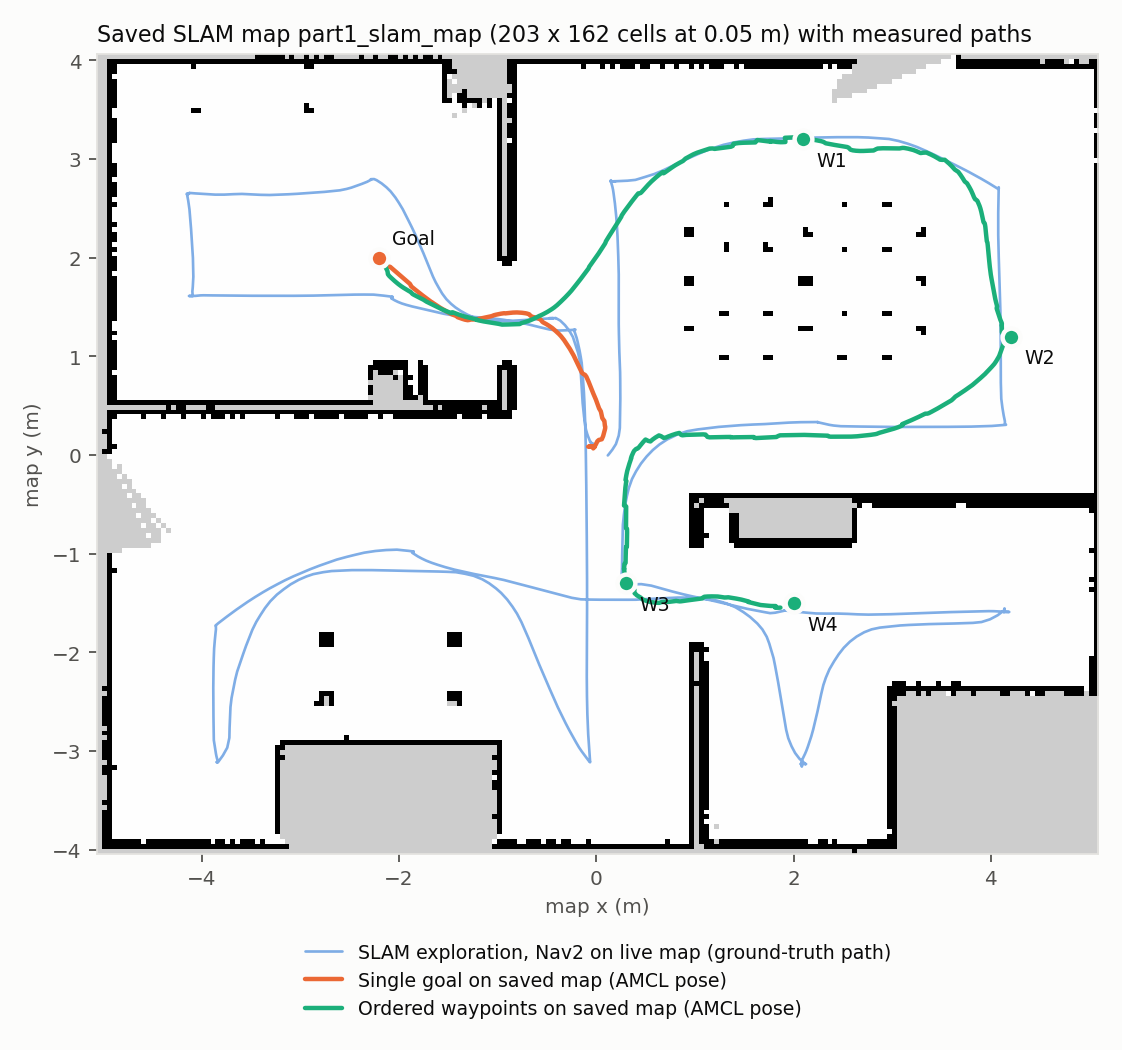
\includegraphics[width=.80\linewidth,height=56mm,keepaspectratio]{figures/part1/slam_map_navigation.png}
\captionof{figure}{Saved SLAM map and measured paths. Mapping covers the house; localization/navigation reload the saved map. The 4:33.8 Part 1 video shows ROS commands, Gazebo control, LiDAR/map views, saving and navigation.}
\end{center}
\textbf{Acceptance and evidence.} The action client requires status 4, an empty missed-waypoint list, a measured arrival at every goal, and a settled final error below 0.25\,m and 0.25\,rad. The controller targets the tighter 0.15\,m / 0.15\,rad limits. Evidence is under \path{task1_rosorin/evidence/full_slam/}; the README includes all launch, map-save and action-client commands.

\clearpage
\section*{2. Part 1: debugging, controlled tests and limits}
\textbf{Distorted maps.} With the vendor SLAM configuration, mapping produced doubled walls and an oversized map. Disabling loop closure removed large jumps but did not eliminate yaw drift during in-place turns. Increasing odometry penalties bounded the error but left a rotated room. A ray-cast scan comparison against the known wall geometry gave a mean residual of 0.010\,m, consistent with the configured LiDAR noise. It found no obvious time/angle/scale mismatch; this supports investigating SLAM configuration, without proving that every sensor input is exact.

The same recorded exploration data were replayed through five configurations, isolating the effect of each change:
\begin{center}\small
\begin{tabular}{p{.61\linewidth}rr}\toprule
Configuration & Mean / max error (m) & Map cells\\\midrule
A: vendor, loop closure on & 2.07 / 5.39 & 274$\times$308\\
B: A, loop closure off & 0.26 / 0.88 & 226$\times$178\\
C: B, stronger odometry penalties & 0.30 / 0.86 & 221$\times$181\\
D: B, minimum travel 0.5\,m / 0.5\,rad & 0.013 / 0.093 & 203$\times$161\\
E: A, minimum travel 0.5\,m / 0.5\,rad (selected) & 0.013 / 0.093 & 203$\times$161\\\bottomrule
\end{tabular}\end{center}
\textbf{Interpretation.} The original minimum-travel thresholds, 0.0\,m and 0.01\,rad, admit many nearly redundant poses while stationary or rotating. With the limited 156$^\circ$ field of view, scan matching and ambiguous loop closures become vulnerable. Restoring 0.5\,m / 0.5\,rad thresholds preserved loop closure and produced a consistent map. This explanation is supported by the replay comparison and the final live run (0.023\,m mean error); it is not a general tuning rule for all robots.

\begin{center}
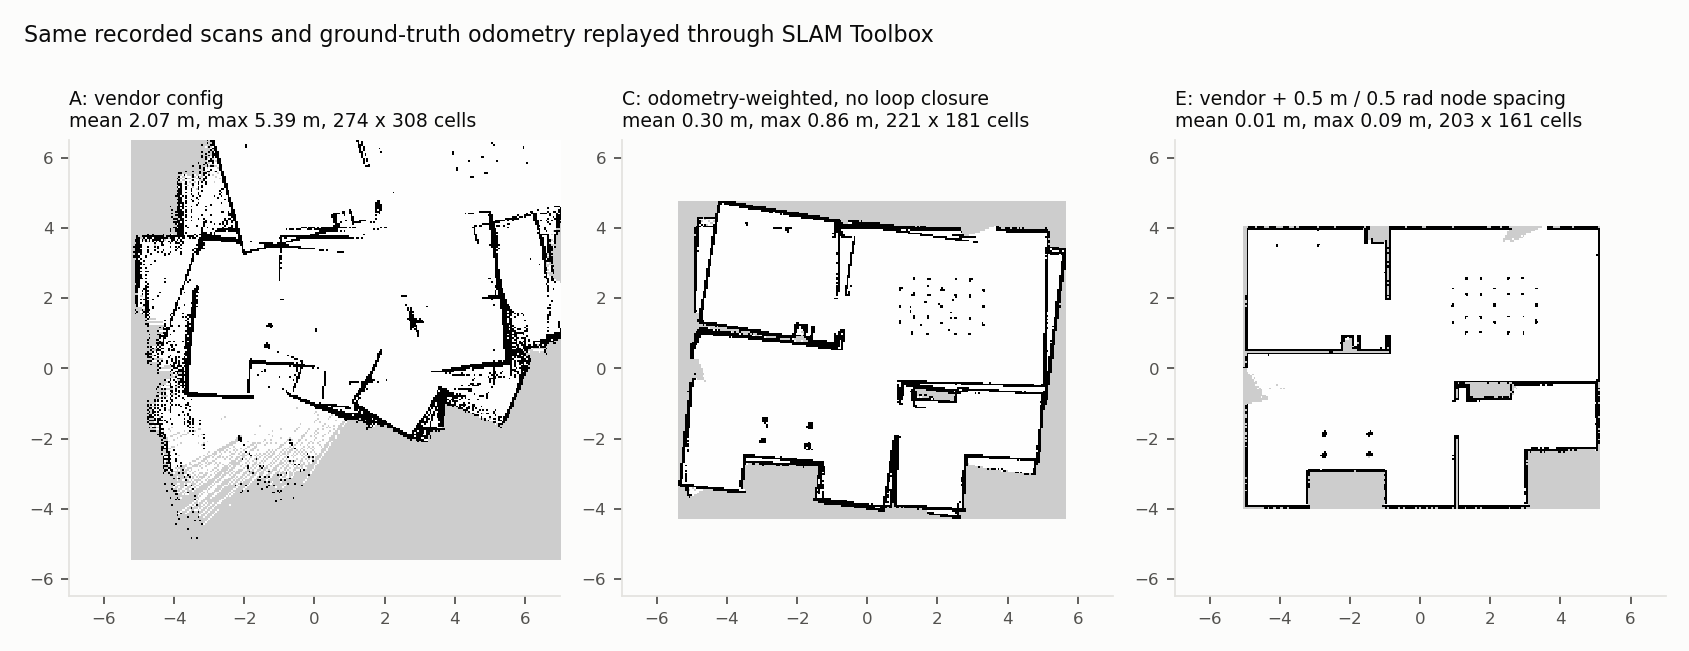
\includegraphics[width=.96\linewidth,height=54mm,keepaspectratio]{figures/part1/slam_replay_maps.png}
\captionof{figure}{Maps reconstructed from the same recording. The final threshold change resolves the large distortions seen in the vendor configuration. Replay parameters, maps and pose-error traces are preserved in \texttt{evidence/slam\_replay/}.}
\end{center}

\textbf{Controller stalls.} DWB repeatedly stalled when a goal lay behind a thin wall, despite a valid path through the doorway; one route incurred 16 progress-checker failures. Adding a static local costmap layer alone did not fix it. RPP followed the global path, but the first trial detected a collision near dining chairs. Wider global inflation (0.30 $\rightarrow$ 0.55\,m), lower scaling (10 $\rightarrow$ 3) and a shorter lookahead (0.4\,m) improved clearance. On a fresh-spawn README rerun, single goal, four waypoints and the U-turn regression route all passed with zero progress-checker failures. Final errors were 0.151/0.144/0.122\,m respectively.

\textbf{Timing and ownership.} Fast-DDS logs showed lost service responses during heavy startup load; AMCL sometimes never activated. The action client now checks lifecycle state, retries service calls and initializes AMCL only after activation. Recovery actions are explicitly recorded; final runs needed none. An unconditional static map-to-odom transform was removed, and duplicate odometry was separated. Drive parameters were corrected from the vendor values to the model's 0.04\,m wheel radius and 0.16/0.18\,m track dimensions; measured forward motion improved from 0.080 to 0.1005\,m for a 0.10\,m command.

\textbf{Limits.} Ground-truth odometry makes SLAM easier than hardware; wheel slip and drift are absent. Rendering runs at roughly 0.53--0.75$\times$ real time. The static world and a few repeated routes do not establish reliability in dynamic clutter. Selected raw results and failure logs, detailed notes and a short VM boot-recovery record are retained; final assembly did not rerun the full ROS experiment.

\clearpage
\section*{3. Research understanding: two routes to coordination}
\textbf{MoManipVLA (CVPR 2025) [2].} Fixed-base vision-language-action models do not directly coordinate a mobile base with an arm. The paper reuses a pretrained VLA as an end-effector waypoint generator and transfers its policy through whole-body motion planning. A predicted waypoint is transformed from the current base frame into the world frame. Planning trades off reachability, trajectory smoothness and collision clearance:
\[
\mathcal O=\lambda_1\mathcal F_r+\lambda_2\mathcal F_s+\lambda_3\mathcal F_c,\qquad
\mathcal F_r=\begin{cases}N_{IK}/N_{max},&\text{IK converges}\\C_0,&\text{otherwise.}\end{cases}
\]
\[
\mathcal F_s=\sum_t\bigl(\|\theta^{t+1}-\theta^t\|_2+\|x_b^{t+1}-x_b^t\|_2\bigr),\quad
\mathcal F_c=\sum_{t,j}\max(0,\epsilon_0-D(q_j^t)).
\]
A bi-level optimizer first searches base poses that induce a promising arm search space, then selects the end-effector path. Dual Annealing with SLSQP refinement reduces the difficulty of joint base/arm search. Its contribution is a planner-based transfer mechanism that avoids learning a whole-body joint policy from scratch. The original paper reports 15.8\% overall success on OVMM, versus 11.6\% for its strongest listed baseline; these are literature results, not this submission's scores.

\textbf{HoMMI (RSS 2026) [3,4].} Whole-body robot teleoperation data are expensive. HoMMI augments bimanual handheld UMI grippers with egocentric sensing to collect robot-free human demonstrations. Egocentric context enables navigation and active perception, but introduces human-to-robot visual and kinematic differences. Its policy addresses these with 3D head-camera features, arm masking, a gripper-centric representation and a relaxed head action: a 3D look-at point, rather than a human's full 6-DoF head pose. A constraint-aware whole-body controller realizes the hand/gaze trajectories on the robot. This contributes both a scalable data interface and a policy/control representation for cross-embodiment transfer. Its paper reports Laundry/Delivery/Tablescape success rates of 90/85/80\% on RB-Y1; none is claimed as reproduced here.

\begin{center}\small
\begin{tabular}{p{.22\linewidth}p{.35\linewidth}p{.35\linewidth}}\toprule
Aspect & MoManipVLA & HoMMI\\\midrule
Learning source & Pretrained fixed-base VLA; limited task adaptation & Robot-free human demonstrations; task policy training\\
Policy output & End-effector waypoint & Bimanual trajectories, widths and look-at point\\
Coordination & Bi-level trajectory search & Constraint-aware differential IK / QP\\
Scene representation & VLA images and ESDF for planning & Wrist features and 3D egocentric features\\
Embodiment focus & Single arm plus mobile base & Bimanual robot, torso, base and active neck\\
Central risk & Wrong waypoint or infeasible local motion & Human/robot mismatch, gaze limits and prediction ambiguity\\\bottomrule
\end{tabular}\end{center}

\textbf{Common lesson.} Both separate task-level intent from robot constraints. MoManipVLA adapts where the base should move to make a waypoint feasible; HoMMI designs transferable hand/gaze actions and lets a controller allocate body motion. Constraint awareness helps execution, but cannot guarantee correct intent, collision-free progress or adequate perception.

\textbf{Experimental questions.} The implementation tests three mechanisms: whether a trained HoMMI policy predicts useful held-out action chunks; whether relaxed head actions reduce kinematic conflict; and whether bi-level planning and its cost terms improve waypoint execution. The studies use different robots, data and metrics, so their numerical scores are not compared against each other or against the full paper benchmarks.

\clearpage
\section*{4. HoMMI: official pipeline and small-scale training}
\textbf{Implementation.} The official repository at commit \artifact{2c002aa} and its pinned UMI/RB-Y1 WBC dependencies are included. The official processing pipeline was run on real Laundry-v3 data: multi-phone grouping/alignment and ArUco gripper calibration, session construction, then replay-buffer construction. Forty raw demonstrations were downloaded; thirty complete demonstrations yielded 17,476 frames and a 3.75\,GB processed replay buffer. A fixed 24/6 demonstration split was used, preventing frames from one demonstration appearing in both training and validation.

\textbf{Reduced training.} The official training entry point and diffusion-policy recipe were retained. To fit the 6\,GB GPU, DINOv3 ViT-B/16 was reduced to ViT-S/16; DiT width/depth to 384/6; head RGB and point-map resolution to 256$^2$; and head tokens to 128. Training used seed 42, batch 8, bf16 and 60 epochs (approximately 10.9k steps, 93 minutes in the recorded run). The historical log reports epoch-mean diffusion loss near 0.31 $\rightarrow$ 0.005 and sampled validation action MSE near 0.080 $\rightarrow$ 0.0029. This MSE is a periodic single-batch diagnostic, not the full validation metric or a robot success rate.

\begin{center}
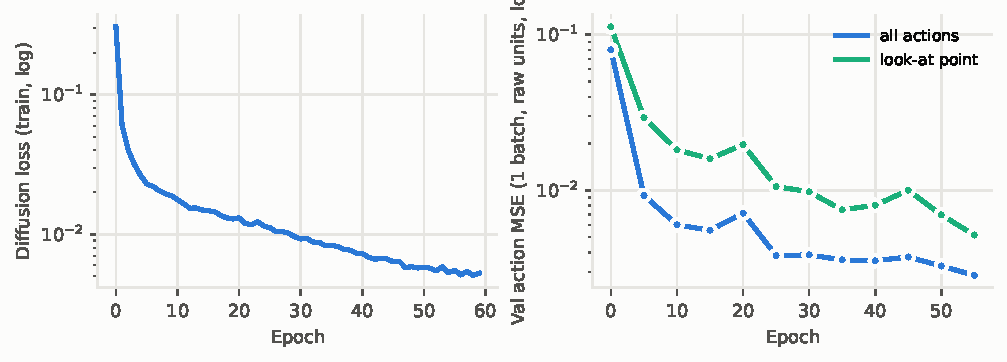
\includegraphics[width=.85\linewidth,height=52mm,keepaspectratio]{figures/part2/hommi_training.pdf}
\captionof{figure}{Recorded training and sampled validation curves. The full JSONL log, resolved configuration and trained checkpoint are bundled. Low training loss alone does not establish closed-loop success.}
\end{center}

\textbf{Offline protocol.} EMA weights with 16 DDIM steps predict 32-step chunks at 20\,Hz (about 1.6\,s). Evaluation uses all 395 sampled windows from the six held-out demonstrations and compares the predictions with future human actions. A hold-still baseline repeats the current state in the same left-gripper frame. The principal metrics are mean Euclidean position/look-at errors, rotation geodesic error and absolute gripper-width error, in physical units.

\begin{center}\small
\begin{tabular}{lrr}\toprule
Chunk-mean error, 395 validation samples & Policy & Hold still\\\midrule
Left gripper position (cm) & 6.65 & 17.87\\
Right gripper position (cm) & 8.71 & 18.25\\
Left gripper rotation (degrees) & 6.00 & 11.65\\
Right gripper rotation (degrees) & 8.69 & 11.94\\
Left gripper width (mm) & 5.14 & 11.54\\
Right gripper width (mm) & 4.37 & 10.37\\
Look-at point (cm) & 22.08 & 31.02\\\bottomrule
\end{tabular}\end{center}
\textbf{Interpretation.} Across the chunk, learned motion is more accurate than holding still. Left-hand error at 0.4\,s is 3.97\,cm versus 9.78\,cm. However, at 0.2\,s the policy is worse for right-hand rotation (6.55 vs 3.81$^\circ$) and gaze position (18.58 vs 13.41\,cm). A plausible explanation is uncertain motion timing and a short two-frame history, rather than uniformly better immediate predictions. The 395 overlapping windows are correlated; six demonstrations remain a small validation set, and no uncertainty estimate treating windows as independent is justified.

\textbf{Pipeline debugging.} DGL installation failed, so a torch FPS shim was used; PyTorch3D transforms reuse the vendored implementation. OpenCV-contrib 4.7.0.72 matches mixed old/new ArUco APIs. A stream-decoding patch avoids loading every full-resolution frame into RAM. Editable installation, LMDB and scikit-learn were added. The patch intends to preserve processing semantics; assembly did not independently establish bytewise equivalence. Training settings and dependency freezes expose these deviations.

\clearpage
\section*{5. HoMMI: head actions, qualitative results and failures}
\textbf{Controller study.} A MuJoCo harness drives the official \artifact{RBY1WholeBodyIK} (Mink/DAQP) and the official look-at solver without the hardware SDK. At each 100\,Hz tick, the IK solution becomes the next measured state: perfect kinematic tracking is assumed. The three modes are \artifact{direct\_lookat}, \artifact{ik} (track a 6-DoF head pose) and \artifact{hold\_init} (fixed neck). Gripper-centric replay evaluates 25 tabletop demonstrations and 30 real Laundry demonstrations, including altered demonstrator head heights.

\begin{center}\small
\begin{tabular}{llrrr}\toprule
Data / zero height offset & Head action & Hand mean (mm) & Hand p95 (mm) & Gaze ($^\circ$)\\\midrule
Tabletop, 25 demos & Look-at & 0.135 & 0.124 & 1.3\\
 & 6-DoF pose & 26.8 & 80.0 & 8.5\\
 & Fixed neck & 0.135 & 0.124 & 19.5\\\midrule
Laundry, 30 demos & Look-at & 0.067 & 0.106 & 4.51\\
 & 6-DoF pose & 2.930 & 11.130 & 5.94\\
 & Fixed neck & 0.067 & 0.106 & 27.54\\\bottomrule
\end{tabular}\end{center}
\textit{Hand p95 is the mean of per-episode 95th percentiles, not a pooled percentile. Values are rounded; exact values are in the CSVs.}

\begin{center}
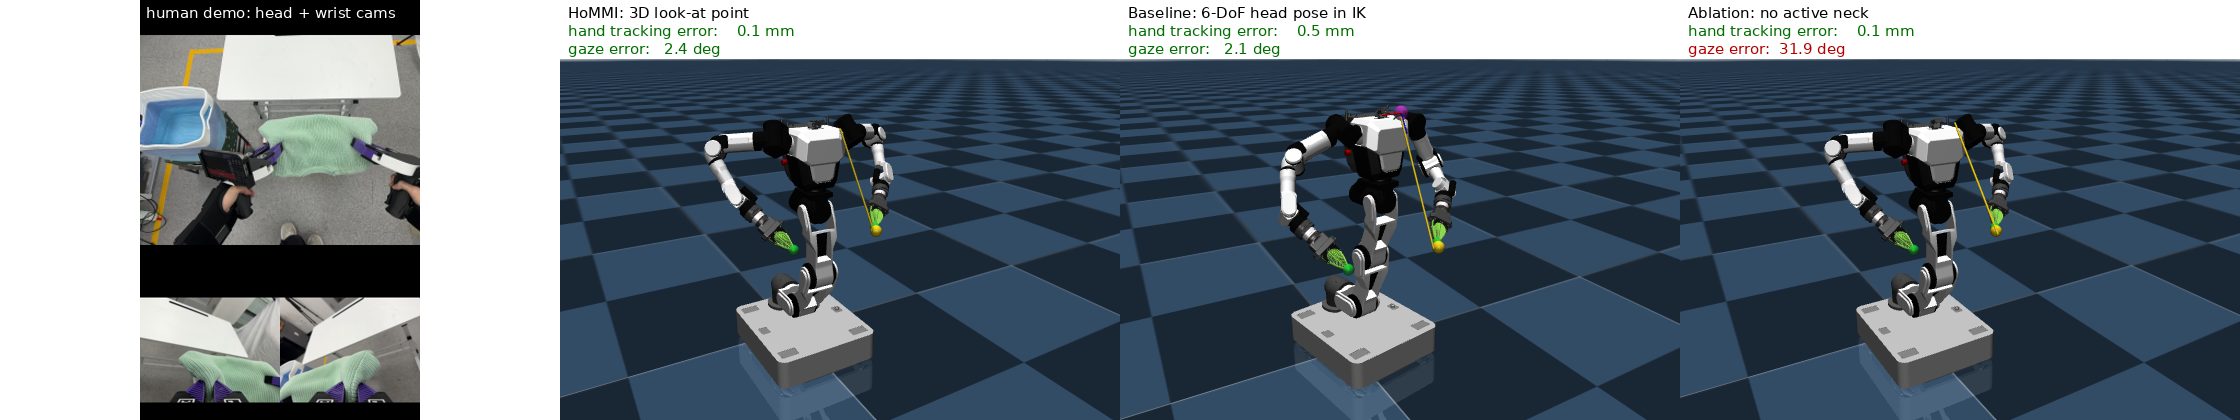
\includegraphics[width=.96\linewidth,height=44mm,keepaspectratio]{../task2_mobile_manipulation/results/hommi_wbc/wbc_laundry_ep0_strip.png}
\captionof{figure}{Human camera views and kinematic RB-Y1 replay with different head actions. Gaze and hand tracking can conflict when the controller tries to match a full human head pose.}
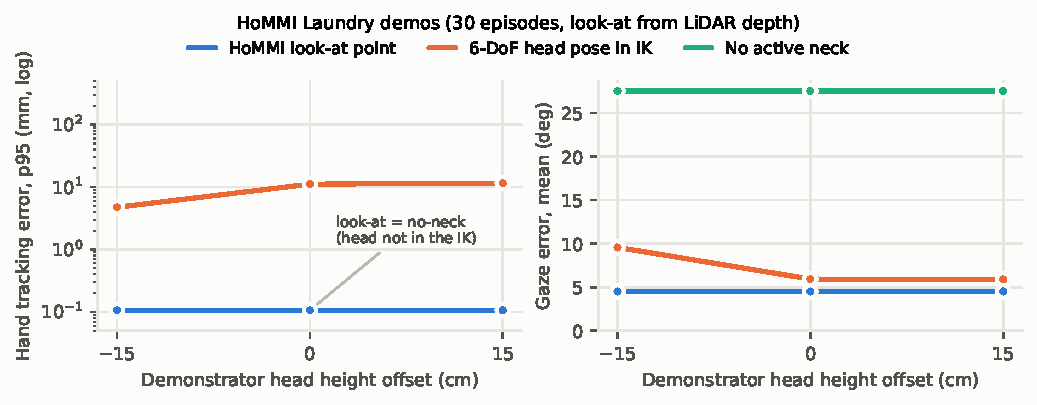
\includegraphics[width=.88\linewidth,height=46mm,keepaspectratio]{figures/part2/wbc_offsets_laundry.pdf}
\captionof{figure}{Laundry replay under different head-height offsets. Look-at preserves hand tracking, while gaze accuracy is constrained by the robot's neck range.}
\end{center}

\textbf{What succeeds.} Relaxed gaze avoids putting an infeasible human head pose in the whole-body IK objective, preserving hand tracking near numerical precision in this idealized harness. A fixed neck preserves hands too, but loses the visual target. Laundry look-at satisfies the study's trackability criterion (hand p95 $<$20\,mm and episode-mean gaze error $<$10$^\circ$) on 23/30 demonstrations at zero offset. This is a trajectory-tracking criterion, not task success.

\textbf{What fails.} Residual gaze errors remain, and the aggregate joint-limit metric shows saturation of relevant hinge joints; it does not isolate the neck. Full 6-DoF head tracking can move the torso to satisfy the human viewpoint at the expense of the hands. The small policy's overlays also show early or delayed cloth/gaze motion and increasing long-horizon errors. Those overlays demonstrate prediction structure, not successful grasping, cloth physics or navigation on an RB-Y1.

\textbf{Potential remedies.} A longer temporal history could disambiguate motion timing; more varied demonstrations and head heights could reduce extrapolation. Gaze planning should account for neck limits and coordinate torso/base movement where hand constraints permit. Contact-rich tasks additionally need physical execution, force sensing or contact feedback. These proposals have not been experimentally validated here.

\clearpage
\section*{6. MoManipVLA: reduced reproduction and improvement}
\textbf{Setup and fidelity.} With no official code used for these experiments, a local implementation models a Panda arm on a 3-DoF holonomic base in procedural MuJoCo table/counter/shelf/stool scenes. It retains reachability via iterative IK, ESDF collision cost, and bi-level Dual Annealing/SLSQP with $\lambda=(10,1,0.6)$ and margin $\epsilon_0=0.1$\,m. Reductions include analytic geometry instead of nvblox, damped-least-squares IK instead of Pinocchio and a much smaller search budget. Crucially, the recorded smoothness term uses \emph{squared} joint/base increments, whereas paper Eq.~4 uses unsquared norms. Results therefore describe this variant, not an exact equation-level reproduction.

\textbf{Protocol.} The main experiment uses evaluation seeds 1000--1059, 60 episodes per variant, oracle waypoints with per-axis position noise $\sigma=8$\,mm and yaw noise 3$^\circ$. Heuristic base placement precedes manipulation. Success requires the implementation's IK, collision and grasp/place alignment checks; grasp execution is kinematic, with no contact dynamics. The oracle exposes target information unavailable to a real VLA; it isolates planning, not perception generalization.

\begin{center}\small
\begin{tabular}{lrrrr}\toprule
Variant & Pick (\%) & Success & SR (\%), 95\% Wilson CI & Latency (s)\\\midrule
Fixed-base waypoint policy & 21.7 & 1/60 & 1.7 [0.3, 8.9] & 0.011\\
Heuristic base placement & 55.0 & 15/60 & 25.0 [15.8, 37.2] & 0.007\\
Direct search & 80.0 & 36/60 & 60.0 [47.4, 71.4] & 5.417\\
Bi-level search & 73.3 & 32/60 & 53.3 [40.9, 65.4] & 6.183\\
Bi-level, no reachability & 1.7 & 0/60 & 0.0 [0.0, 6.0] & 17.988\\
Bi-level, no smoothness & 71.7 & 33/60 & 55.0 [42.5, 66.9] & 5.960\\
Bi-level, no collision cost & 8.3 & 2/60 & 3.3 [0.9, 11.4] & 15.057\\
Bi-level + feasibility-first & 78.3 & 40/60 & 66.7 [54.1, 77.3] & 5.079\\\bottomrule
\end{tabular}\end{center}
\textbf{Findings.} Reachability and collision terms are essential in this setup. Removing smoothness changes success by only one episode, providing no evidence of a success-rate gain. Direct search is faster and has higher observed success here than bi-level search: the original paper's bi-level advantage is not reproduced. Latencies are recorded Python CPU times per planning waypoint and are far from real-time control.

\textbf{Failure analysis and tested fix.} In the bi-level variant, 22/60 episodes end with base/furniture collision. A continuous soft collision hinge can trade penetration against reachability improvements. The proposed change selects the minimum-cost candidate among already evaluated collision-free, IK-feasible candidates; if none exists, it falls back to the original argmin. It adds no candidate evaluations. On paired seeds it rescues 8 episodes and breaks none (two-sided exact McNemar $p=0.0078125$); success rises 32/60 $\rightarrow$ 40/60 and base collisions fall 22/60 $\rightarrow$ 13/60. This is a local empirical improvement with no global safety guarantee.

\begin{center}
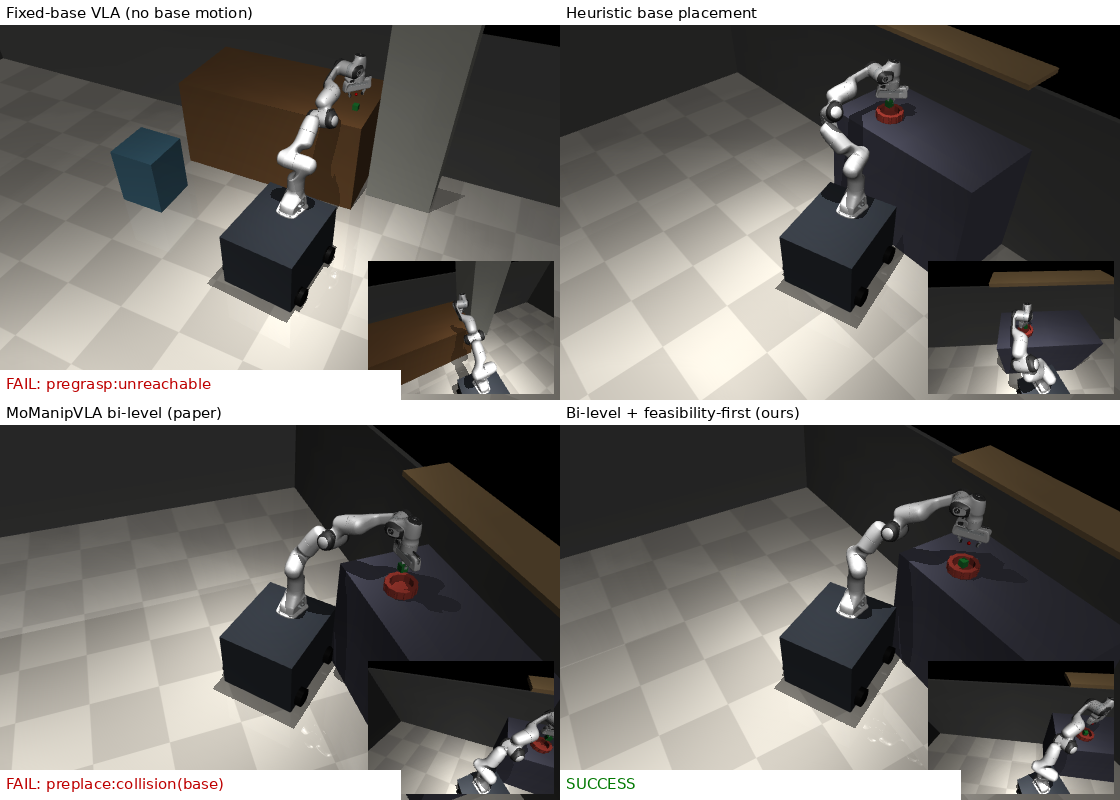
\includegraphics[width=.98\linewidth,height=40mm,keepaspectratio]{../task2_mobile_manipulation/results/momanipvla/episode_1007.png}
\captionof{figure}{Seed 1007: fixed base is unreachable, heuristic placement collides with the shelf, the original bi-level selection collides with the counter, and feasibility-first succeeds. Seed 1014 remains a failure with a blocking stool in the local search window.}
\end{center}
\textbf{Waypoint quality.} On 40 seeds, bi-level success drops from 60\% to 50/30/5\% as oracle noise rises from 0 to 8/16/30\,mm. A separately trained DINOv3-S plus three-layer transformer waypoint head (300 expert episodes, two instruction embeddings) has about 5.5\,cm validation error and 0/40 mobile successes. It is a small visual waypoint surrogate, not OpenVLA-7B. Its workspace regression bias exposes a transfer failure; a planner cannot repair an incorrect semantic target.

\clearpage
\section*{7. Reproducibility, submission audit and conclusions}
\textbf{Review entry points.} The top-level README maps every deliverable to files. Task-specific READMEs contain installation, launch/training/evaluation commands and assumptions. The seven-page report covers both parts. \path{videos/part1_demo.mp4} lasts 273.828\,s (within 3--5 minutes); \path{videos/part2_demo.mp4} presents controller replay, policy predictions, planning success and failure cases. The Part 2 video interleaves actual GNOME Terminal commands and outputs for HoMMI inference, MoManipVLA evaluation and WBC replay with the corresponding visualizations. Online copies are in the \href{https://drive.google.com/drive/folders/10DDnV1l6JCk7svF_ktngK9A5h_L9aIn2?usp=sharing}{Google Drive folder (videos and report)}. The Part 1 video shows ROS commands alongside Gazebo/RViz results.

\textbf{Three levels of reproduction.}
\begin{enumerate}
\setlength\itemsep{2pt}
\item \emph{Artifact review:} run \path{task2_mobile_manipulation/scripts/audit_results.py} to recompute rates, paired tests and offline errors from CSV/NPZ files. Run \path{report/validate_submission.py} to check required files, links, maps/configuration consistency, report length and video metadata. No robot or GPU is needed.
\item \emph{Small reruns:} the bundled 792\,MB HoMMI checkpoint and six held-out samples support official-policy inference without the full replay buffer. A compact 30-episode plan plus recorded look-at depths supports WBC replay. Short simulation/inference outputs are recorded separately under verification paths; they do not replace historical aggregates.
\item \emph{Complete reruns:} the pinned 404-file download manifest reconstructs the HoMMI raw subset; the official patched pipeline rebuilds the full replay buffer and trains the small policy. All MoManipVLA evaluation seeds and variants are specified. A clean ROS Humble/Fortress machine or the vendor VM can build the two included ROS packages and replay the mapping/navigation instructions.
\end{enumerate}

\textbf{Provenance and portability.} Vendored official code and robot assets preserve their licenses and pinned revisions. Selected raw logs and failure evidence, per-episode CSVs, per-sample errors, training configuration, dependency freezes and representative plots are included. Original absolute training paths remain in provenance records, while review scripts resolve paths from their own location and full evaluation accepts a dataset/cache override. The learned waypoint checkpoint is copied to the location its inference class actually reads. DINOv3 access may require license acceptance and an authenticated model download; no credentials are bundled. Full raw videos, the 3.75\,GB training replay buffer, duplicate training checkpoints and VM disks are omitted, with reconstruction commands provided.

\textbf{Statistical and practical limits.} Sixty procedural episodes give broad confidence intervals; success changes are paired by seed. Evaluation on six held-out demonstrations does not establish household generalization. The small waypoint-head trainer did not explicitly fix all random seeds; diffusion sampling and GPU kernels can also vary across reruns. Checkpoints permit inference without retraining. MuJoCo replay assumes ideal tracking, no grasp/contact dynamics and exact scene geometry. ROS mapping uses ground-truth odometry. These choices keep the experiments feasible on the available computer, but limit transfer claims.

\textbf{Conclusions.} The submission demonstrates the required ROS control, sensing, SLAM, map saving and both navigation modes, with reproducible evidence of debugging. HoMMI's small official policy improves chunk-average held-out action error over holding still, while its relaxed head action reduces kinematic conflict in replay. The reduced MoManipVLA experiment shows both the value and the limits of constraint-aware planning: feasible-candidate selection helps a soft-cost planner, but waypoint bias and blocked local search still cause failures. Future validation should combine hard collision constraints, broader temporal context and closed-loop physical execution; these are proposed extensions, not completed results.

\vfill
\textbf{References and primary resources}\par
\small
[1] Hiwonder, \emph{ROSOrin Pro: Gazebo Simulation}.\newline
\url{https://wiki.hiwonder.com/projects/rosorin-pro/en/latest/docs/9_Gazebo_Simulation.html}\par
[2] Z. Wu, Y. Zhou, X. Xu, Z. Wang and H. Yan, \emph{MoManipVLA: Transferring Vision-language-action Models for General Mobile Manipulation}, CVPR 2025.\newline
\url{https://arxiv.org/abs/2503.13446}\par
[3] X. Xu et al., \emph{HoMMI: Learning Whole-Body Mobile Manipulation from Human Demonstrations}, RSS 2026. DOI: 10.15607/RSS.2026.XXII.205.\newline
\url{https://roboticsproceedings.org/rss22/p205.html}\par
[4] Official HoMMI code: \url{https://github.com/xxm19/hommi}; paper: \url{https://arxiv.org/abs/2603.03243}; data: \url{https://huggingface.co/datasets/real-stanford/hommi}.\par
[5] Robot model: \url{https://github.com/google-deepmind/mujoco_menagerie}; Nav2: \url{https://docs.nav2.org/}; SLAM Toolbox: \url{https://github.com/SteveMacenski/slam_toolbox}.
\end{document}
